\section{Metropolis-Hastings \\ MCMC (linear model)}

Write a simple MetropolisHastings MCMC to fit the data from linfit data.npz to the linear function
\begin{equation}
    f(\Vec{x}|\Vec{a})=a_0 + a_1\Vec{x}
\end{equation}

Plot up the joint posterior probability distribution for the two parameters as well as marginalized posterior probabilities for each parameter. Clearly describe your process for obtaining a
good acceptance rate through tuning the average step sizes via your proposal distributions.
Overplot the joint 68.3\% and 95\% confidence intervals for the two parameters.

\begin{figure}
    \centering
    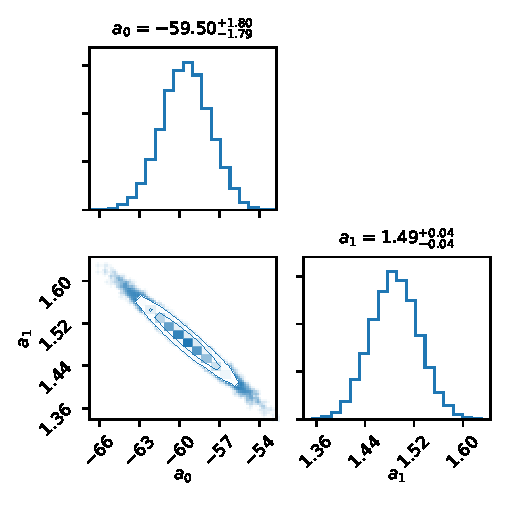
\includegraphics[0.5\textwidth]{CodeAndFigures/LinearModelMetropolisHastings.pdf}
    \caption{Caption}
    \label{fig:LinearHastings}
\end{figure}